\section{Selección de Herramientas}
\subsection{Selección de motor de Base de Datos}
Actualmente existe una gran cantidad de oferta de sistemas de bases de datos, aunque en modelo de base de datos mas habitual es el relacional, que se vincula estrechamente con el \textbf{lenguaje SQL}.
\subsubsection{Base de Datos Relacionales}
Las bases de datos relacionales se basan en almacenar, relacionar, consultar y tranferir datos dentro de tablas y registros de tuplas. Las tablas se relacionan entre si por medio de campos compartidos y se pueden establecer muchas relaciones entre las mismas formando un entramado de datos super-organizado y estructurado.

Se puede decir que al principal problema de las bases de datos relacionales es precisamente que al crecer el volumen de datos suelen crecer las estructuras (Scale Up) y se convierten en verdaderos laberintos de conexiones que hacen que la organización y gestión de los datos pueda llegar a ser pesada y ralentice las famosas Queries así como la transmisión de datos.

Otro problema importante de estas bases de datos es que al cambiar la estructura de una sola tabla puede provocar impacto en otras muchas, cualquier variación supone un coste en compatibilidad, tiempo y recursos.
\subsubsection{Base de Datos Documentales}
Las bases de datos documentales tales como MongoDB o PostgreS centran su valor en almacenar los datos en documentos en lugar de tablas, estos \textbf{documentos} son recipientes de datos en un formato semi-estructurado, que permite que en un mismo tipo de recipiente se almacene distintos tipos de datos en un mismo tipo de elementos. Por lo tanto se podría decir que las bases de datos documentales tienen la ventaja de ser super-flexibles, se adaptan a los cambios y tienen optimizacion de consultas en base de datos para grandes cantidades de datos.

Este objetivo de este proyecto es monitorear el manejo de un conductor, lo que esto conlleva que se hará uso de una gran cantidad de datos, haciendo las Bases de Datos Documentales ideales para este propósito, para la etapa del desarrollo del prototipo se propone el uso de MongoDB para el almacenamiento de datos del manejo (almacenaje de datos del lado del servidor) y SQlite como almacenamiento interno de los datos propios de la aplicación.
\subsection{Selección de herramientas para el servicio Web}
Básicamente se usara el servicio Web para el entrenamiento y predicción de patrones de manejo del conductor, por lo que es necesario encontrar una herramienta que se adecue a este propósito.
A continuación se detallaran algunos puntos principales por lo que se decidió usar el lenguaje de programación Python en esta etapa.
\subsubsection{Usado por?}
Python es utilizado por programadores que quieren profundizar en el análisis de datos o aplicar técnicas estadísticas, y por desarrolladores que recurren a datos científicos.
\subsubsection{Usabilidad}
La codificación y la depuración es más fácil de hacer en Python, principalmente debido a la sintaxis "agradable", ademas cualquier pieza de funcionalidad siempre se escribe de la misma manera en Python lo que no es igual en otras herramientas como por ejemplo R.
\subsubsection{Flexibilidad}
Python es flexible para hacer algo nuevo que nunca se haya hecho antes. Los desarrolladores también pueden usarlo para crear scripts en un sitio web u otras aplicaciones.
\subsubsection{Fácil de aprender}
El enfoque de Python en legibilidad y simplicidad hace que su curva de aprendizaje sea relativamente baja y gradual.
Python se considera un buen lenguaje para iniciar programadores.
\subsubsection{Uso en el análisis de datos}
Python se usa generalmente cuando las tareas de análisis de datos deben integrarse con aplicaciones web o si el código de estadísticas debe incorporarse en una base de datos de producción.
\subsubsection{Librerías populares}
\begin{itemize}

\item \textbf{Pandas} para manipular datos fácilmente.

\item \textbf{SciPy / NumPy} para la informática científica.

\item \textbf{sckikit} aprende a utilizar los métodos de aprendizaje automatico.

\item \textbf{matplotlib} para hacer gráficos.

\item \textbf{statsmodels} para explorar datos, estimar modelos estadísticos y realizar pruebas estadísticas y pruebas unitarias.
\end{itemize}
\subsection{Selección de herramientas para la aplicación móvil}
La aplicación móvil para el monitoreo del manejo de conducción requiere el uso de uno o mas sensores propios del dispositivo móvil, por lo que se vio optimo el uso de desarrollar la misma de manera nativa, mas propiamente dicha en \textbf{Android nativo} debido a que este tipo de aplicaciones tienen menos capas para poder llegar las funcionalidades propias del dispositivo móvil para realizar una acción, por lo tanto si se desea acceder a la cámara, GPS o sensores del dispositivo, el código esta optimizado para que la funcionalidad se lleve a cabo rápidamente.

Entre otras ventajas de desarrollo de aplicaciones nativas se pueden nombrar las siguientes:
\begin{itemize}
\item Mejor rendimiento
\item Menor consumo de memoria
\item Mayor velocidad
\item Aprovechamiento total del hardware del dispositivo(Camara, GPS, Sensores, entre otros).
\end{itemize}

\subsection{Selección de metodología}
\subsubsection{Metodología de la Investigación}

La \textbf{metodología de la investigación} es una disciplina de conocimiento encargada de elaborar, definir y sistematizar el conjunto de técnicas, métodos y procedimientos que se deben seguir durante el desarrollo de un proceso de investigación para la producción de conocimiento.

Orienta la manera en que vamos a enfocar una investigación y la forma en que vamos a recolectar, analizar y clasificar los datos, con el objetivo de que nuestros resultados tengan validez y pertinencia, y cumplan con los estándares de exigencia científica.

La \textbf{metodología de la investigación}, en este sentido, es también la parte de un proyecto de investigación donde se exponen y describen razonadamente los criterios adoptados en la elección de la metodología, sea esta \textbf{cuantitativa} o \textbf{cualitativa}.
\begin{itemize}
\item \textbf{Metodología cuantitativa}
La metodología cuantitativa es aquella empleada por las ciencias naturales o fácticas, que se vale de datos cuantificables a los cuales accede por observación y medición.

Para su análisis, procede mediante la utilización de las estadísticas, la identificación de variables y patrones constantes. Su método de razonamiento es deductivo, para lo cual trabaja con base en una muestra representativa del universo estudiado.

Por lo tanto para el cumplimiento del objetivo se hará el uso de una metodología de investigación cuantitativa  debido al análisis de datos que se requiere.

\end{itemize}

\section{Proceso de desarrollo}

\subsection{Especificación de requisitos}
El presente proyecto conlleva una serie de requisitos funcionales explícitos y otra serie de requisitos no funcionales implícitos los cuales son presentados a continuación:

\subsubsection{Requisitos funcionales}
Los requisitos del presente proyecto constan de     módulos principales con un serie de funcionalidades requeridas.

El la tabla CUADRO 3.1  se puede observar una columna con el nombre principal del modulo, otra columna con las funcionalidades requeridas para dicho modulo y una columna de descripción de cada una de las funcionalidades.


\begin{table}[h!]
\begin{center}
\begin{tabular}[c]{|p{4cm}|p{4cm}|p{6cm}|}
\hline
\textbf{MODULO} & \textbf{FUNCIONALIDAD REQUERIDA} & \textbf{DESCRIPCIÓN}\\
\hline 
\textbf{Gestión de usuarios} & Creación de cuentas de usuario & La creacion de cuentas como prerrequisito de acceso a la aplicación\\
\hline 
&Ingreso a la aplicación&Para mantener la privacidad de los datos del usuario, el acceso a la aplicación se realiza mediante un ingreso con nombre de usuario  y contrasenia.\\
\hline 
\textbf{Captura de datos}&Lectura de sensores&Captura de datos de sensores necesarios para encontrar patrones de manejo en la conducción de un especifico usuario.\\
\hline 
&Envio y almacenaje de datos al servidor&Captura y almacenaje de datos de los sensores en el servidor.\\
\hline 
\textbf{Entrenamiento}&Captura de datos de entrenamiento&Almacenaje de datos en el servidor para su posterior  entrenamiento.\\
\hline
&Generación de un modelo de predicción&Generar un modelo de predicción con los datos de entrenamiento proporcionados y un algoritmo de aprendizaje no supervisado.\\
\hline
\textbf{Predicción}&Predecir si un patrón es anómalo o no&Con el modelo generado en la fase de entrenamiento determinar si el conductor conduce de manera correcta o anómala según el entrenamiento proporcionado previamente.\\
\hline
\textbf{Alertas}&Consultar capacidad de conducción&Consultar estado del conductor en caso de que el sistema encuentre un patrón anómalo en la conducción\\
\hline
&Enviar notificaciones contactos de emergencia&En caso de que el conductor no pueda confirmar que se encuentra capaz de seguir conduciendo el sistema enviara notificaciones de alerta a los contactos de emergencia del conductor con la ubicación GPS del mismo.\\
\hline
\textbf{Incrementar el aprendizaje}&Agregar nuevos datos a la rutina de conducción&En caso de que el conductor confirme que se encuentra conduciendo bien, previa consulta realizada se procederá a incrementar este patrón al modelo de predicción.\\
\hline

\end{tabular}
\caption{\textbf{Requerimientos funcionales}}
\end{center}
\end{table}

\subsubsection{Requisitos no funcionales}
Estos requisitos son aquellos que aunque no estan especificados en el trabajo, son indispensables en el desarrollo del mismo.

\begin{itemize}
\item \textbf{Entorno de desarrollo y compilación }
El desarrollo de la aplicación se llevará a cabo usando Android Studio como entorno de desarrollo con las herramientas necesarias para la creación de aplicaciones en toda clase de dispositivos Android.
\item \textbf{Control de versiones de código fuente}
Se usará un sistema de control de versiones para el código fuente de la
aplicación de tipo GIT, el elegido es Gitlab, ya que no obliga a hacer público el repositorio.
\item \textbf{Persistencia de datos}
Los datos de la aplicación deben almacenarse en un sistema, para ello se hará uso de un backend en el que se almacenarán los objetos necesarios.
\item \textbf{Lenguaje de programación}
Para desarrollar de forma nativa para Android se utilizará el lenguaje de
programación Java, requisito imprescindible para tal fin.
\item \textbf{Entorno de ejecución}
Se proporcionará un ejecutable en formato apk para poder instalar en dispositivos Android.
\item \textbf{Pruebas}
Se realizarán las pruebas unitarias con JUnit y los test de usuario que resulten necesarios.
\item \textbf{Documentación}
Se proporcionara un Documento Final y diapositivas explicativas del modo de uso de la aplicación móvil.
\end{itemize}

\subsection{Plan de trabajo}
A continuacion se detalla de forma resumida los objetivos y entregables de cada fase.
\begin{enumerate}[1.]
\item \textbf{Plan de trabajo}
\textit{Objetivos: }Definir el proyecto y realizar su planificación inicial.
\textit{Entregables: }Plan de trabajo.
El plan de trabajo servirá como guía para el resto del desarrollo.
\item \textbf{Análisis, diseño y prototipo}
\textit{Objetivos: }Realizar el análisis de tareas, diseño y prototipo.
\textit{Entregables: } Documentación que incluye escenarios de uso, diagramas de flujo de interacción y un prototipo de alto nivel.
\item \textbf{Implementación}
\textit{Objetivos: }Implementar la solución del proyecto y documentación complementaria.
\textit{Entregables: }Código fuente, instalables y documentación complementaria.
Es la fase final del proyecto en la que se obtiene el producto final. Puede requerir iterar con las fases anteriores en caso de detectar problemas en el producto.
\item \textbf{Entrega final}
\textit{Objetivos: }Finalizar el proyecto y documentarlo.
\textit{Entregables: }Documento y diapositiva de presentación del proyecto.
En esta fase se finalizará la fase anterior en caso de no haberlo hecho y se presentará al público objetivo nuestro producto.
\end{enumerate}
\subsection{Prototipo}

Para instalar la aplicación se debe tener la apk en el dispositivo móvil, y también tener habilitado la opción orígenes desconocidos como se muestra en la Figura 3.1.
\begin{figure}[h!]
  \begin{center}	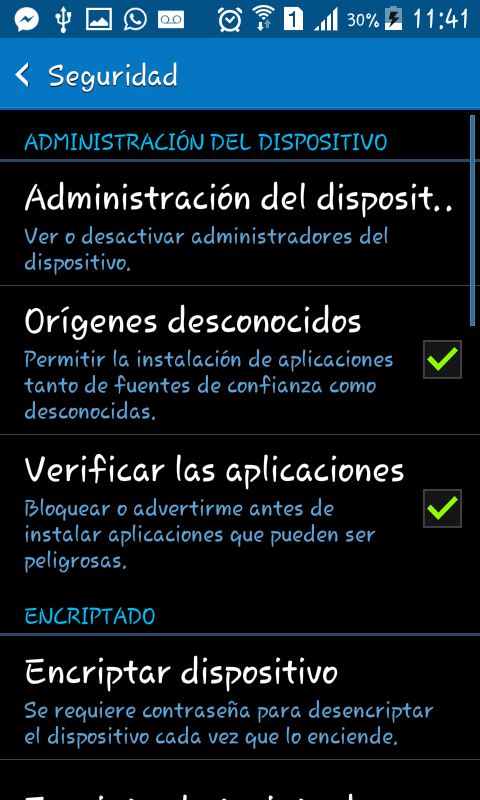
\includegraphics[width=0.4\textwidth]{imagenes/origenesdes}
  \caption{Habilitar orígenes desconocidos}
  \end{center}
\end{figure}
A continuación se muestran pantallas del prototipo inicial.
\begin{itemize}

\item \textbf{Icono de la aplicación}

Una vez instalada la aplicación se puede observar en el dispositivo un nueva aplicacion denominada "Driving App" como se puede ver en la Figura 3.2.

\begin{figure}[h!]
  \begin{center}	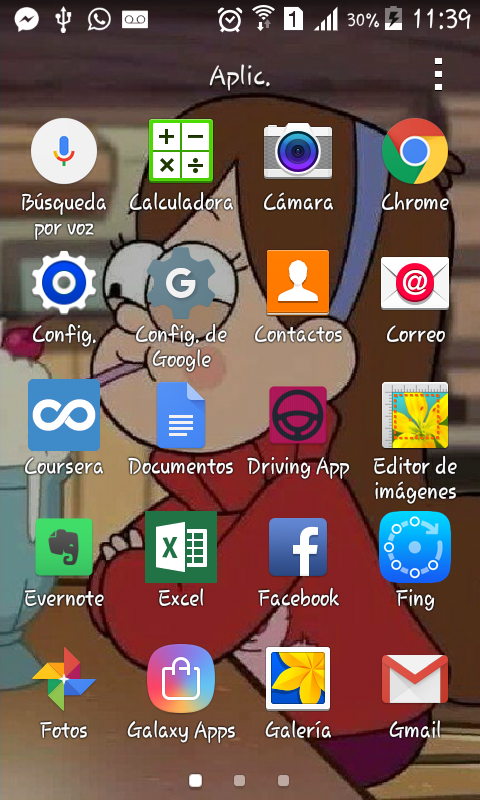
\includegraphics[width=0.4\textwidth]{imagenes/iconoapp}
  \caption{Icono de la aplicación}
  \end{center}
\end{figure}

\item \textbf{Ingreso a la aplicación}
Al abrir la aplicacion se puede observar una pantalla de logueo como se muestra en la Figura 3.3.; donde para ingresar a la misma se pone "root"  como nombre de usuario y "123" como contrasenia.
\begin{figure}[h!]
  \begin{center}	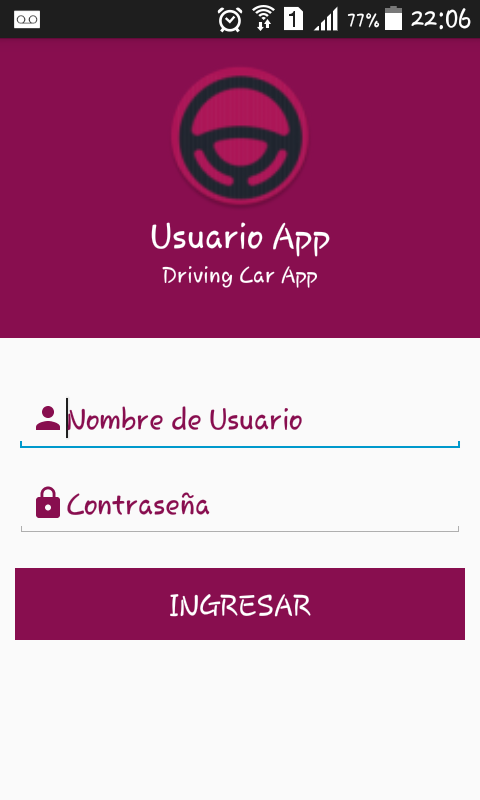
\includegraphics[width=0.4\textwidth]{imagenes/inicio}
  \caption{Ingreso a la aplicación}
  \end{center}
\end{figure}

\item \textbf{Pantalla principal}
La pantalla principal consta de un boton (Ver Figura 3.4)el cual sirve para empezar a guardar los datos (de manera local en el prototipo) de conducción (datos capturados del acelero metro en la etapa de prototipo).
\begin{figure}[h!]
  \begin{center}	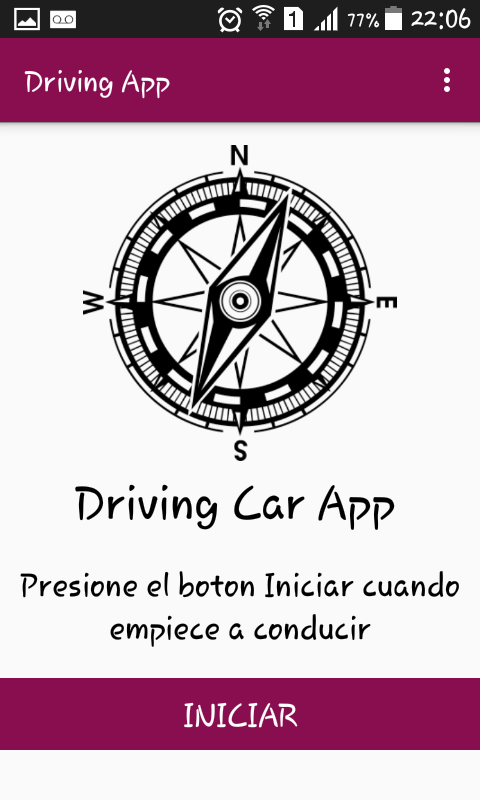
\includegraphics[width=0.4\textwidth]{imagenes/principal}
  \caption{Pantalla principal de la aplicación}
  \end{center}
\end{figure}
\item \textbf{Menú}
El menú consta de dos opciones que se detallaran mas adelante(Ver Figura 3.5).
\begin{figure}[h!]
  \begin{center}	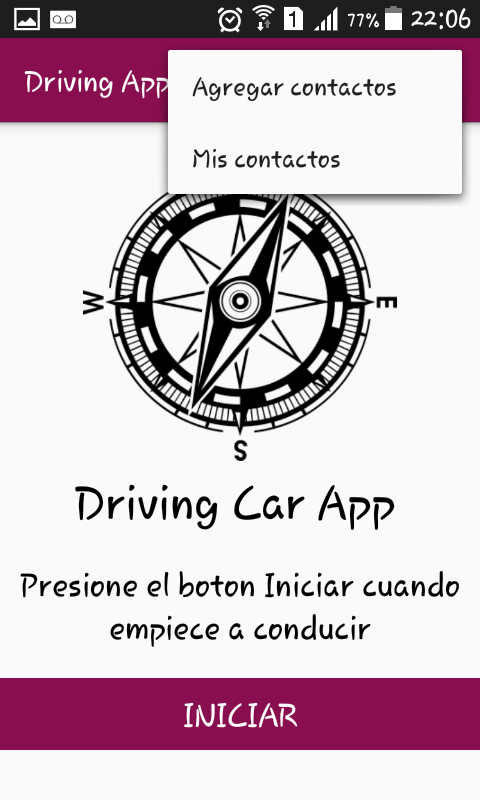
\includegraphics[width=0.4\textwidth]{imagenes/menu}
  \caption{Menú de la aplicación}
  \end{center}
\end{figure}

\item \textbf{Funcionalidad agregar contactos}
Esta funcionalidad se habilita al presionar en el menú la opción "Agregar contactos"; consta de agregar contactos de emergencia para el usuario, su aparencia es como se muestra en la Figura 3.6.
\begin{figure}[h!]
  \begin{center}	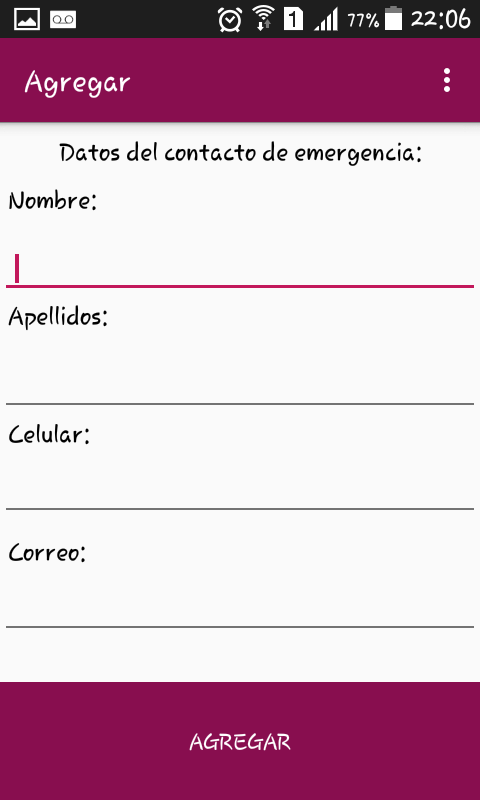
\includegraphics[width=0.4\textwidth]{imagenes/agregar}
  \caption{Opción agregar contactos}
  \end{center}
\end{figure}
\item \textbf{Listar contactos}
Esta funcionalidad se habilita al presionar en el menú la opción "Mis contactos"; consta en listar los contactos de emergencia para el usuario, su aparencia es como se muestra en la Figura 3.7.
\begin{figure}[h!]
  \begin{center}	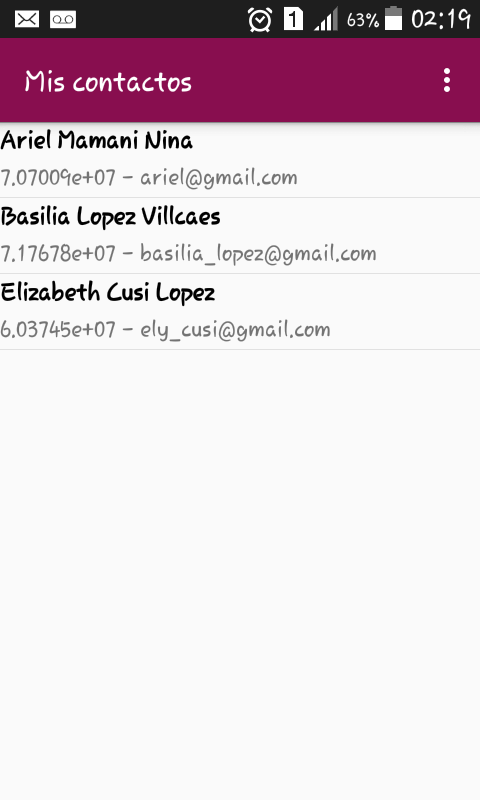
\includegraphics[width=0.4\textwidth]{imagenes/lista}
  \caption{Opción mis contactos}
  \end{center}
\end{figure}
\end{itemize}